\section{Exercise 2}
\subsection*{2.1}
If we denote the pixels in the image \textit{I} as \textit{x'} and \textit{y'} and we denote the pixels in $\tilde{I}$ as \textit{x} and \textit{y}, we can map the pixels in $\tilde{I}$ to the pixels in $I$ by taking each pixel pair, \textit{x} \textit{y}, augment with a 1, and then multiply with the inverted transformation matrix:
\begin{equation*}
	\begin{bmatrix}
		x'\\
		y'\\
		1
	\end{bmatrix} = \left(
	\begin{bmatrix}
		1&0&t_x\\
		0&1&t_y\\
		0&0&1
	\end{bmatrix} \cdot
	\begin{bmatrix}
		cos(2\pi-\theta)&-sin(2\pi-\theta)&0\\
		sin(2\pi-\theta)&cos(2\pi-\theta)&0\\
		0&0&1
	\end{bmatrix} \cdot
	\begin{bmatrix}
 		s&0&0\\
 		0&s&0\\
 		0&0&1
 	\end{bmatrix} \right)^{-1}	\cdot
	\begin{bmatrix}
		x\\
		y\\
		1
	\end{bmatrix}
\end{equation*}
The resulting augmented pixel pair, \textit{x'} \textit{y'}, are then the corresponding x and y coordinates in the image $\textit{I}$. Running through all pixels in $\tilde{I}$, performing this mapping and then copying the pixel value from $I$ to $\tilde{I}$ would result in the correct transformation.\\
We can also compute the inverted transformation matrix. Multiplying the three transformation matrices results in the following matrix:
\begin{equation*}
	\begin{bmatrix}
		s\cdot cos(2\pi-\theta)&s\cdot -sin(2\pi-\theta)&t_x\\
		s\cdot sin(2\pi-\theta)&s\cdot cos(2\pi-\theta)&t_y\\
		0&0&1
	\end{bmatrix}
\end{equation*}
To invert this matrix we need to perform 4 steps. In the first step we compute the matrix of minors. That is, for each entry in turn, we ignore the current row and current column, and then compute the determinant of the remaining elements which then replaces the entry we are at in the matrix. In step two we then change sign of all the elements so we get a checkerboard pattern of positive and negative values. This is the matrix of cofactors. In step three we transpose the cofactors matrix. And in the last step we multiply all elements with $\frac{1}{det} = \frac{1}{(s\cdot cos(2\pi-\theta))^2+(s\cdot -sin(2\pi-\theta)-(s\cdot sin(2\pi-\theta)))}$. We then get the matrix:
\begin{equation*}
	\frac{1}{det} \cdot 
	\begin{bmatrix}
		s\cdot cos(2\pi-\theta)&-(s\cdot -sin(2\pi-\theta)&(s\cdot -sin(2\pi-\theta)\cdot t_y)-(s\cdot cos(2\pi-\theta)\cdot t_x)\\
		-(s\cdot sin(2\pi-\theta)&s\cdot cos(2\pi-\theta)&(s\cdot cos(2\pi-\theta)\cdot t_y)-(s\cdot sin(2\pi-\theta)\cdot t_x)\\
		0&0&(s\cdot cos(2\pi-\theta))^2-(s\cdot sin(2\pi-\theta)\cdot s\cdot -sin(2\pi-\theta))
	\end{bmatrix}
\end{equation*}

\subsection*{2.2}
\begin{figure}[H]
	\begin{subfigure}[b]{0.45\linewidth}
		\centering
		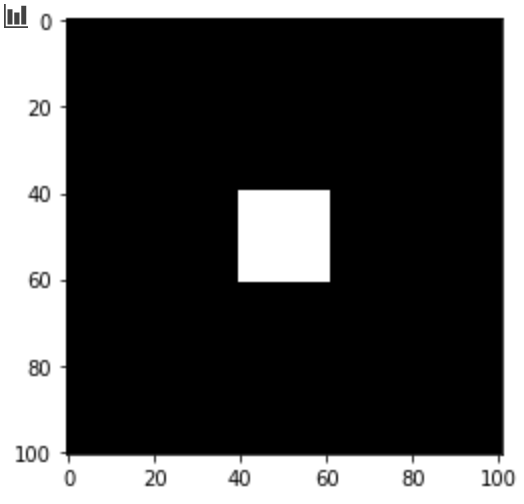
\includegraphics[width=\linewidth]{Materials/E2/before}
		\caption{Before transformation}
	\end{subfigure}
	\hfill
	\begin{subfigure}[b]{0.45\linewidth}
		\centering
		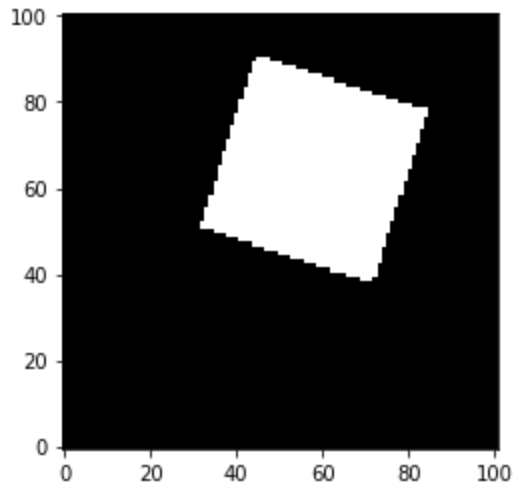
\includegraphics[width=\linewidth]{Materials/E2/res}
		\caption{After transformation}
	\end{subfigure}
	\caption{Before and after transformation of white square.}
	\label{transformation}
\end{figure}
In \autoref{transformation} we see the white square before and after the transformation. In \autoref{E2code} we see the code used for this exercise. We first define the transformation matrices in homogenous coordinates and then dot them all together, and then we take the inverse of this matrix as he final transformation matrix. We then loop through all pixels in the output image and map them to the input image through the inverted transformation matrix. To make the dotting of the transformations work, we use 3x3 matrices, and thus the input coordinates needs to be augmented with a third coordinate equal to 1. The output coordinate is also augmented, and to convert back to Cartesian coordinates we thus divide the \textit{x} and \textit{y} coordinates with the augmented output coordinate, however, this augmented output coordinate is always 1, so we simply just get the \textit{x} and \textit{y} coordinate. To accommodate the nearest neighbour interpolation, we simply round the coordinates. After we have performed the transformation, we plot the new square where we have changed the direction of the y-axis to be of correct orientation.

\begin{figure}[H]
	\centering
	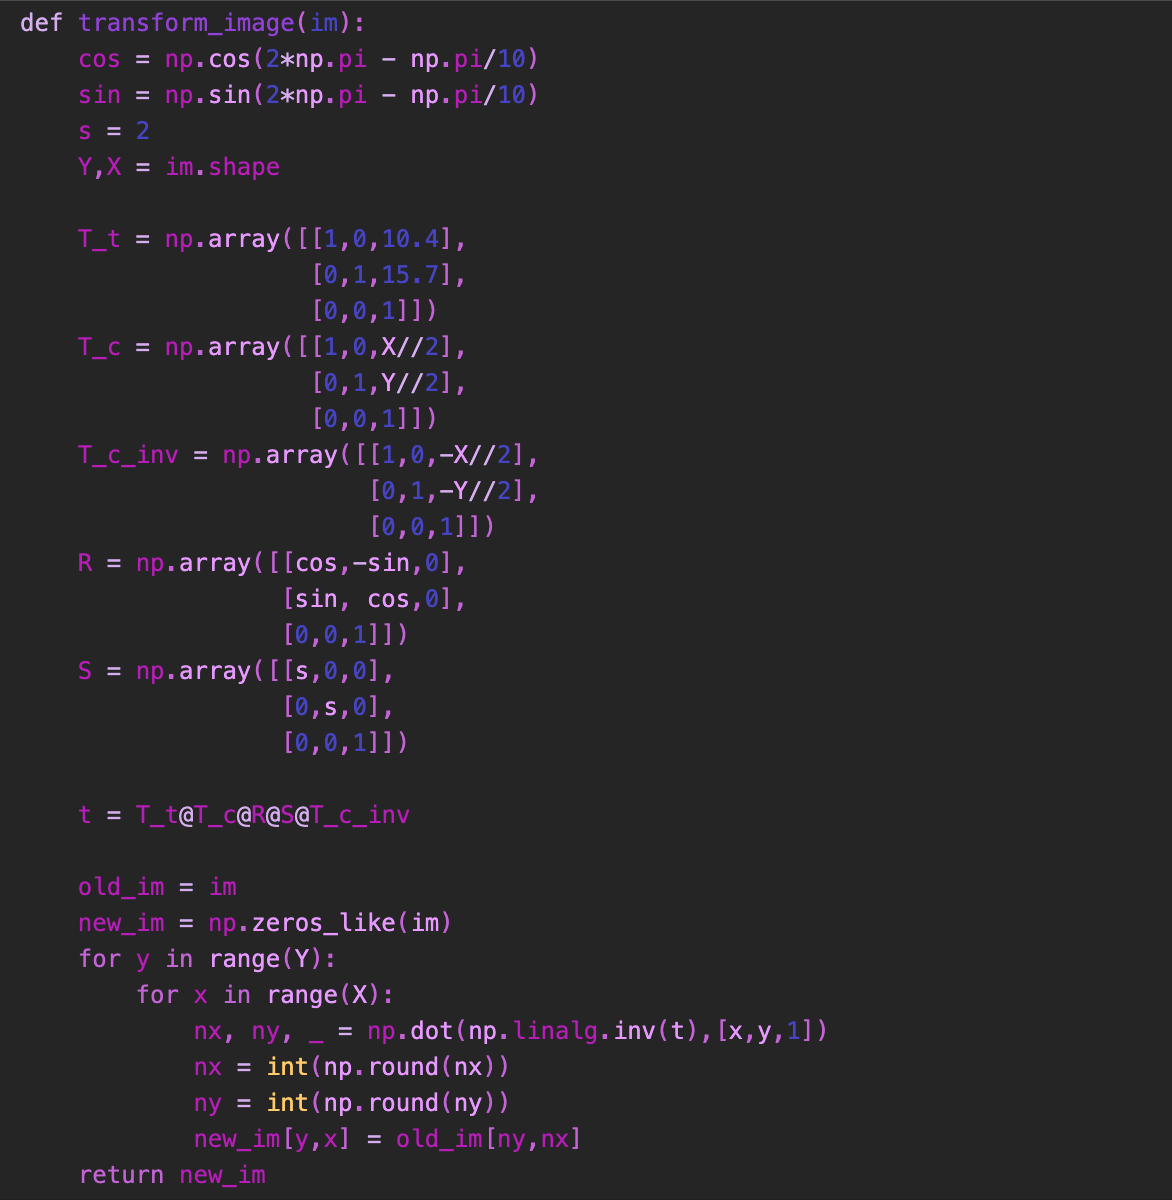
\includegraphics[width=\linewidth]{Materials/E2/code}
	\caption{Code used for this exercise.}
	\label{E2code}
\end{figure}